\documentclass{article}%
\usepackage[T1]{fontenc}%
\usepackage[utf8]{inputenc}%
\usepackage{lmodern}%
\usepackage{textcomp}%
\usepackage{lastpage}%
\usepackage[head=40pt,margin=0.5in,bottom=0.6in]{geometry}%
\usepackage{graphicx}%
%
\title{\textbf{Crisis en la frontera de EEUU es real según la secretaria de Seguridad Nacional}}%
\author{AP}%
\date{07/03/2019}%
%
\begin{document}%
\normalsize%
\maketitle%
\textbf{URL: }%
http://www.eluniversal.com/internacional/34942/secretaria{-}seguridad{-}nacional{-}crisis{-}en{-}la{-}frontera{-}es{-}real\newline%
%
\textbf{Periodico: }%
EU, %
ID: %
34942, %
Seccion: %
internacional\newline%
%
\textbf{Palabras Claves: }%
NO\_TIENE\newline%
%
\textbf{Derecho: }%
2.1%
, Otros Derechos: %
\newline%
%
\textbf{\textit{"Enfrentamos una crisis, una crisis real, grave y sostenida en nuestras fronteras", dijo la secretaria de Seguridad Nacional de EEUU, Kirstjen Nielsen en una audiencia de la Comisión de Seguridad}}%
\newline%
\newline%
%
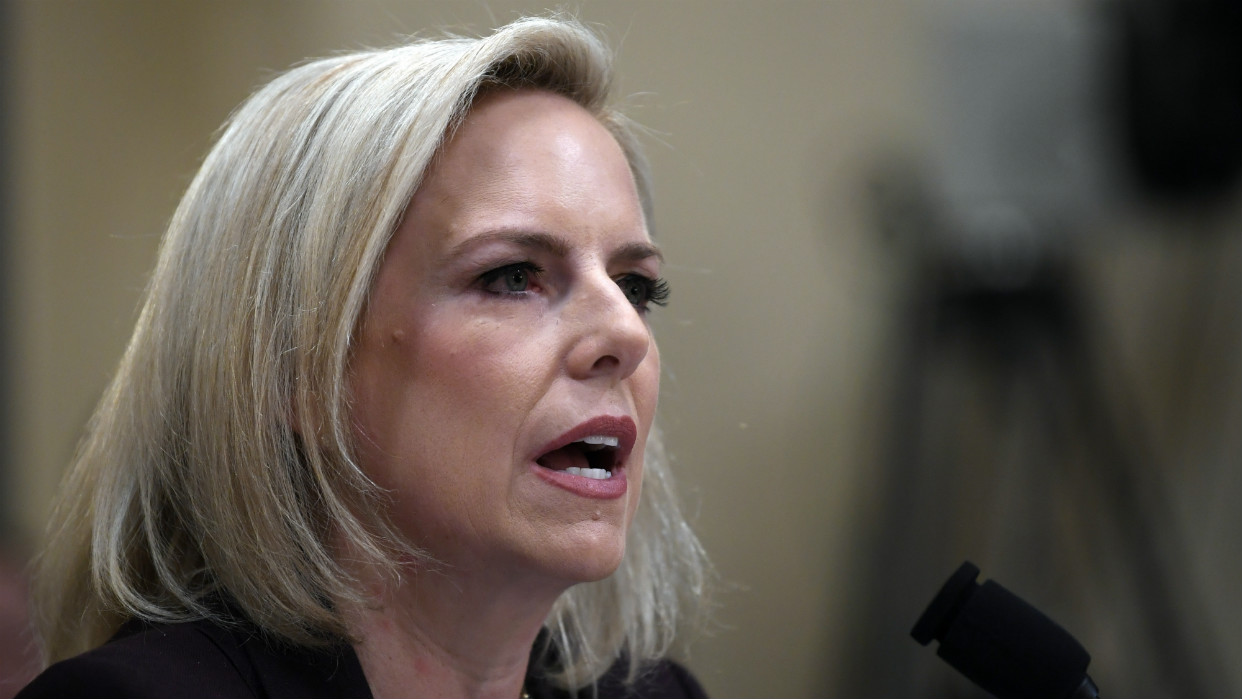
\includegraphics[width=300px]{EU_34942.jpg}%
\newline%
%
Washington.{-} La secretaria de Seguridad Nacional estadounidense, Kirstjen Nielsen, hizo hincapié el miércoles en que la crisis en la frontera con México no es una fabricación, al responder a preguntas de legisladores demócratas por primera vez desde que éstos ganaron la mayoría en la cámara baja.%
\newline%
%
"Enfrentamos una crisis, una crisis real, grave y sostenida en nuestras fronteras", dijo en una audiencia de la Comisión de Seguridad Nacional. "Que nadie se equivoque: esta cadena de miseria humana se agrava", indicó AP.%
\newline%
%
El presidente de la comisión, Bennie Thompson, dijo que el objetivo de la audiencia era en parte darle a Nielsen la oportunidad de iniciar una “discusión seria” en lugar de repetir las declaraciones del presidente Donald Trump sobre una crisis de seguridad en la frontera, y revelar qué sabía sobre las separaciones de familias el año pasado. Dijo que la supervisión de la frontera estaba muy retrasada.%
\newline%
%
“No hay palabrerío que cambie el hecho de que ella sabía que el gobierno de Trump aplicaba una política de separación de familias en la frontera”, dijo Thompson. “Para peor, el gobierno chapuceó la aplicación de su plan cruel, al perder el rastro de los niños e incluso deportar padres a Centroamérica sin sus hijos”.%
\newline%
%
Se preguntó a Nielsen si conocía las consecuencias psicológicas de separar a niños de sus padres y con cuánta anticipación se enteró de la política de “tolerancia cero” que condujo a la separación de más de 2.700 niños de sus padres el año pasado. También se le preguntó sobre sus conversaciones con Trump cuando el presidente declaró una emergencia nacional en la frontera para obtener fondos para el muro que se propone construir entre Estados Unidos y México.%
\newline%
%
“Hay una emergencia”, dijo Nielsen. “He visto poblaciones vulnerables. Esta es una verdadera crisis humanitaria permitida por el sistema. Debemos cambiar las leyes”.%
\newline%
%
La secretaria de prensa de la Casa Blanca, Sarah Sanders, hizo su aporte a través de Twitter: “La crisis en nuestra frontera no es un secreto”, escribió. Los demócratas “optaron por ignorarla”.%
\newline%
%
La audiencia era una de tres dedicadas a la inmigración en el Congreso el miércoles. Desde que tomaron el control de la cámara, los demócratas han dado prioridad a la investigación de las separaciones de familias y exigido la presentación de los documentos respectivos.%
\newline%
%
Mientras Nielsen declaraba ante la cámara, el comisionado de Aduanas y Fronteras, Kevin McAleenan, presentaba diapositivas ante la Comisión Judicial del Senado para destacar el número creciente de grupos de al menos 100 personas en zonas remotas como el Bootheel de Nuevo México y Ajo, Arizona, y los retos sin precedentes de brindar atención médica en sus instalaciones de detención a corto plazo.%
\newline%
%
Decenas de miles de familias cruzan la frontera sin autorización todos los meses, lo cual agota los recursos. El mes pasado las detenciones de migrantes sumaron más de 76.000, el doble que en el mismo período del año pasado. Y según Nielsen, el pronóstico es que el problema se agravará al mejorar el tiempo.%
\newline%
%
Se prevé que el Senado votará la semana próxima y rechazará la declaración de emergencia nacional de Trump como ya lo hizo la cámara. Sin embargo, se da por sentado que Trump vetará la medida y el asunto probablemente se resolverá en los tribunales.%
\newline%
%
El principal contralor interno de Seguridad Nacional, John Roth, también declaraba el miércoles, lo mismo que James McHenry, un funcionario del Departamento de Justicia que supervisa las cortes de inmigración. El jueves, agentes de Aduanas y Protección Fronteriza declararán sobre el reclutamiento de agentes y un contrato por 297 millones de dólares con la consultora Accenture. Esta firma reclutó apenas dos agentes durante los primeros 10 meses del contrato.%
\newline%
%
\end{document}